
 \section{Validation of Primary Findings} % (fold)
 \label{sec:results}


%OUTLINE:
%\begin{enumerate}
%\item \cmark~Introduce MASE.
%\item \cmark~WPE is a good measure of predictability.  %Figure: best athlete MASE vs.
%its WPE.
%\item \cmark~Talk about structure analysis. Just because %there is forward information
%transfer, does not mean that linear predictors can get at %this.
%\subitem \cmark~For this show a figure of (a) ARIMA vs MASE %(b) LMA vs MASE in a side by%
%side plot.
%\item full results.  Image: MASE vs. WPE for both LMA \& %ARIMA.  Points to make:
%\begin{enumerate}
%\item \cmark~clusters are distributed differently
%\item \cmark~clusters are shaped differently---tight or not
%\item \cmark~clusters move differently between LMA and ARIMA
%\item finally, the diagonal line is important. If you're %below it, you could do
%better.
%\end{enumerate}
%\end{enumerate}

%BRAINSTORMING 
%\begin{itemize}
%\cmark\item The kind of complexity present matters, i.e., that is whether the complexity is structured or not.[[use here and mention in intro]] 
%\cmark\item Quantifying structured and unstructured complexity is nontrivial in the case of real-valued noisy time series but WPE does this. [[talk about again here but justify in information theory section]]
%\item Maybe plot a big chunk of \col and a big chunk of \gcc together and show that they both look complex. 

%\cmark\item \gcc appears visually very complex, *and* according to WPE this complexity is unstructured. And a constant, linear and nonlinear prediction strategy all fail. We should be able to conclude that guessing random values is the best we can do as is shown by MASE [[Use in this section]]

%\cmark\item \col is also complex (can even be chaotic/ point to CHAOS paper) but the complexity is structured according to WPE and as such that complexity is usable for prediction [[use in this section]]

%\cmark\item \col brings about the point nicely that some prediction strategies cannot utilize the processes internal information transfer method. That is a nonlinear internal information transfer system cannot be predicted effectively with a linear strategy. This gives a practitioner leverage on when to give up and when to keep working. [[use in this section as bridge to next section]]

%\end{itemize}


In this section we validate the two key primary findings of this work which we introduced in Section \ref{sec:intro}:



\begin{enumerate}

\item The existence of predictable structure in noisy real-valued time series is quantifiable by WPE and as a result WPE is correlated with prediction accuracy (MASE) of an ideal predictor. 

%\subitem [[Simply reminders not to be included]]WPE can quantify when a noisy real-valued time series is predictable.[[I am unsatisfied with predictable in this sentence, need a better word to say "better than random walk" or ``able to be forecast effectively" or ``has the structural capacity to transmit information in a way that the time series can be effectively forecast"

%\item The existence of complex structure in a noisy real-valued time series is quantifiable and this type of complexity is directly correlated with predictability

\item The way structure/information/complexity is processed internally by a given process plays a crucial role in predictability.


%\subitem [[Simply reminders not to be included]]We will have shown that the existence whether linear or nonlinear is picked up on with WPE but this point gets at whether the prediction model can use the structure or not (linear can't use nonlinear structure). The right to left shifts in \col and some of the \svd regimes and the lack of shift in \gcc illustrate this nicely.

%\subitem [[Simply reminders not to be included]]This is the linear vs nonliear vs random we see with the right to left shifts with lower complexity time series. 

\end{enumerate}



%This portion should justify the following claim%%%%%%%%%%%%%%%%%%%%%%
%\item The existence of predictable structure in noisy real-valued time series is quantifiable by WPE and as a result WPE is correlated with prediction accuracy (MASE)  
%%%%%%%%%%%%%%%%%%%%%%%%%





%\item First paragraph: WPE is a good measure of predictability.  Figure:
%best athlete MASE vs. its WPE. 


%\item Quantifying structured and unstructured complexity is nontrivial in the case of real-valued noisy time series but WPE does this. [[talk about again here but justify in information theory section]]

As we discussed in Section \ref{sec:meaComplex} distinguishing structured from unstructured complexity in the case of real-valued time series is non trivial, i.e., distinguishing when a complex signal omits predictable structure and when the signal is effectively random is not a trivial task. As described in Section \ref{sec:intro}, for a practitioner this can be frustrating because it can be nearly impossible to find the source of faulty predictions: Is it simply that we need to use a more ideal (possibly more advanced) predictor or is it the case that the time series is simply so complex that using a simple (yet inconsistent) forecast strategy such as random walk is the best we can do. Fortunately, weighted permutation entropy (WPE) allows us to make this distinction for noisy real-valued time series. 

In Figure~\ref{fig:pred_vs_wpe} we plot the best prediction (i.e., the lowest MASE over all 3 methods\footnote{LMA,ARIMA,na\"ive} over all 15 runs of that program) for each of the 8 programs under investigation. 
\begin{figure}[htbp]
  \centering
  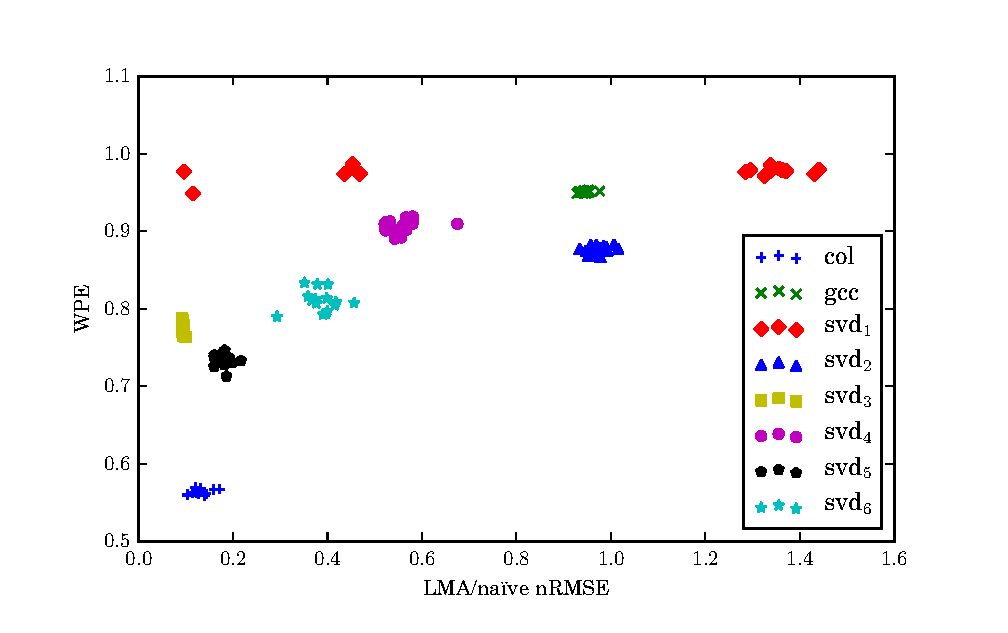
\includegraphics[width=0.75\textwidth]{figs/prediction_vs_entropy}
  \caption{The best MASE among all runs and prediction methods vs weighted
  permutation entropy. For each of these, the word length used is $6$. The
  dashed line is a least-squares linear fit of all the points except for {\tt
  SVD$_1$} which we have excluded for reasons explained in the text.}
  \label{fig:pred_vs_wpe}
\end{figure}
What we see here is that the relationship between prediction accuracy (MASE) and the weighted permutation entropy is much as we conjectured: The existence of predictable structure in noisy real-valued time series as quantified by low to moderate WPE  is correlated with prediction accuracy (MASE) of the ``best"predictor\footnote{We do not claim to have found the ideal predictor for each signal, simply the best predictor over what we used; Which we believe to be a fair sampling of standard prediction techniques for this type of signal.}. We will not further validate this claim through some examples. 


To further validate this finding we present an in-depth analysis of three examples (\col, \svdfive and \gcc ) which nicely cover the range of complexity from low to high respectively. In Figures~\ref{fig:lma_vs_arima} and \ref{fig:arima_pred_vs_ent} we plot the MASE of LMA and ARIMA (respectively) against the weighted permutation entropy of each of the 15 runs of all 8 programs. We also list all of these values in Table \ref{tab:error}

\begin{table}[htdp]
\caption{MASE distributions for 1-step predictions at a 10\% prediction horizon over 15 runs for each signal and average wpe at word length 6 for each signal.}
\begin{center}
\begin{tabular}{|c|c|c|c|c|}
\hline
                   & MASE LMA    & MASE ARIMA &MASE na\"{i}ve   & $l=6$ \\
\hline
\gcc                  & $ 1.5296\pm 0.0214$ & $1.8366 \pm0.0157 $ & $0.9510 \pm 0.0011$ & $0.9430 \pm 0.0013$ \\

\col           & $ 0.0500 \pm0.0018  $ & $0.5989  \pm 0.2114 $ & $0.5707\pm0.0017$&  $0.5131 \pm 0.0034$ \\

\svd Reg. 1     & $ 0.8273\pm 0.0755$ & $ 0.7141\pm 0.0745 $ & $2.6763\pm4.3282$&  $0.9572 \pm 0.0156$ \\
\svd Reg. 2     & $1.2789 \pm0.0196 $ & $2.1626 \pm0.0265 $ &  $3.0543\pm0.0404$ &   $0.8464 \pm0.0044$ \\
\svd Reg. 3       & $0.6192 \pm0.0209 $ & $0.7129 \pm 0.0096 $ & $31.3857\pm 0.2820$ &  $0.7157 \pm 0.0056$ \\
\svd Reg. 4     & $ 0.7789\pm0.0358 $ & $0.9787 \pm0.0321 $ & $2.6613\pm0.0739$ & $0.8246 \pm 0.0077$ \\
\svd Reg. 5     & $ 0.7177\pm 0.0483 $ & $2.3700  \pm 0.0505 $ & $20.8703 \pm 0.1915$&  $0.6776 \pm 0.0068$ \\
\svd Reg. 6     & $ 0.7393\pm 0.0682 $ & $ 1.4379\pm 0.0609$ & $2.1967\pm0.0830$&  $0.7475 \pm 0.0106$ \\
\hline
\end{tabular}
\end{center}
\label{tab:error}
\end{table}%





\begin{figure}[htbp]
  \centering
       
  \begin{subfigure}{0.5\textwidth}
    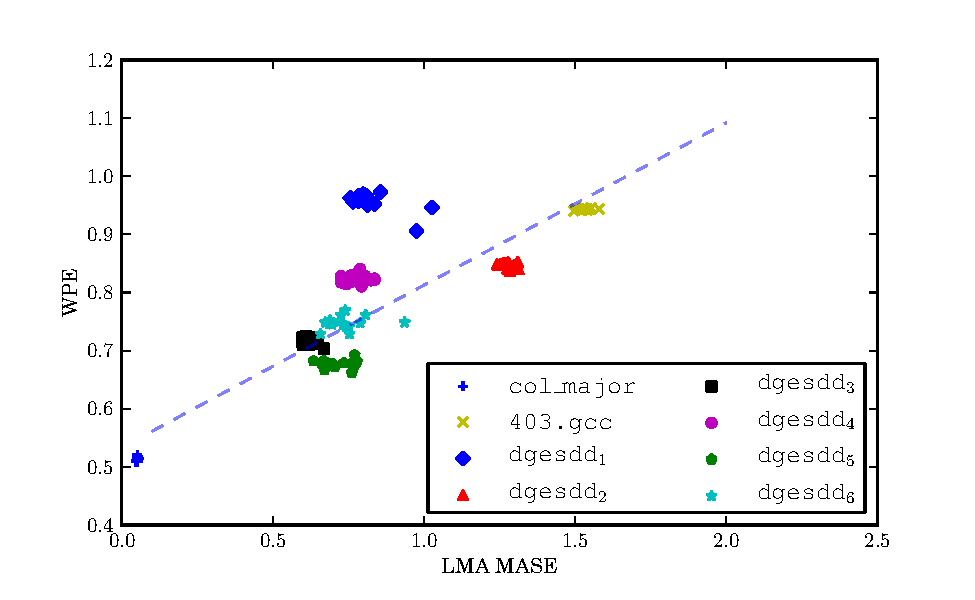
\includegraphics[width=\textwidth]{figs/LMA_prediction_vs_entropy}
    \caption{The MASE of LMA vs weighted permutation entropy. }
    \label{fig:lma_pred_vs_ent}
  \end{subfigure}%
  \begin{subfigure}{0.5\textwidth}
    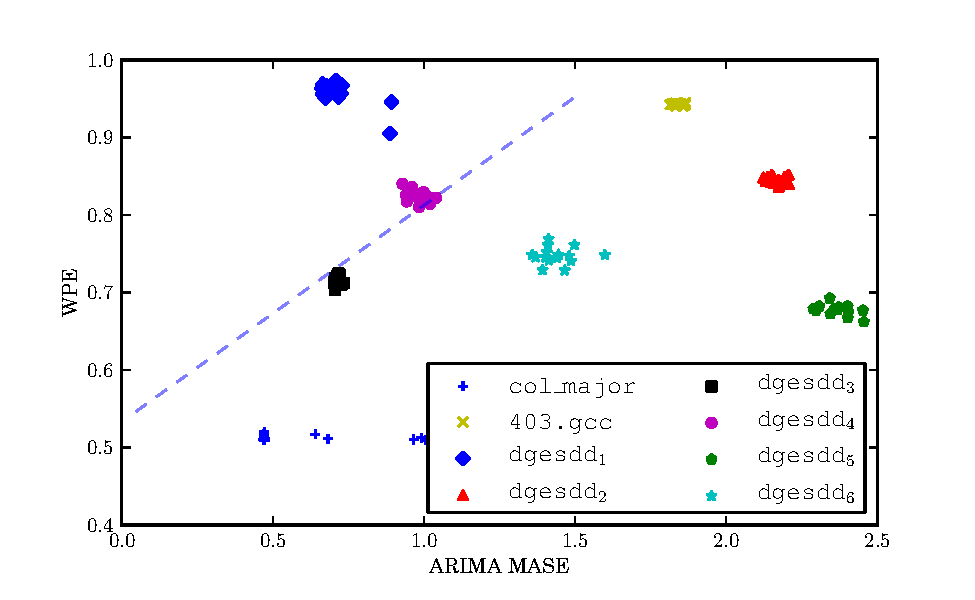
\includegraphics[width=\textwidth]{figs/ARIMA_prediction_vs_entropy}
    \caption{The MASE of ARIMA vs weighted permutation entropy. }
    \label{fig:arima_pred_vs_ent}
  \end{subfigure}
\caption{
For each of these, the word length used is $6$. The MASE values for LMA against ARIMA. The dashed line is the identity, delineating the traces for which either LMA or ARIMA performed better. All traces except those from \svd$_1$ lie above the line, indicating that LMA is better suited prediction method for the computer traces considered.}\label{fig:lma_vs_arima}  
\end{figure} 

We will start with the lowest complexity program: \col. Conceptually this program is very simple but due to computer design choices this program can result in highly complex even chaotic time series traces, see \cite{mytkowicz09}. If we forecast this signal using an out-of-the-box linear forecaster (ARIMA) or an out-of-the-box constant predictor we receive MASE ($0.59 \pm 0.21$ and $0.57 \pm$ 0.001 respectively) which suggest that on average we can only predict this signal twice as well as the simple random walk prediction. This would suggest that there is some predictive structure present but not that much. However, if we quantify the predictive structure present in this signal using WPE we see that this signal is highly structured with a WPE of ($0.51 \pm 0.003$.) The existence of structured which we quantified with WPE implies that an ideal predictor capable of using this signals information should be able to predict this signal much better than the random walk due to the high amount of predictive structure or equivalently the low complexity. This is in fact the case. \col is a complex signal, i.e., chaotic, but it is complex in a structured way. Using a prediction technique that can process nonlinear information yields forecasts with a MASE of $0.05 \pm 0.001$, this is a prediction 20 times more accurate than a random walk forecast. The existence of predictive structure as quantified by WPE could be precisely the information needed to continue searching for an ideal predictor like LMA. 

Maybe even more convincing than a low complexity signal like \col is a moderately complex signal like \svdfive. This signal omits a WPE of $0.677 \pm 0.006$, this is a significantly higher complexity than \col but still implies the existence of a great deal of predictive structure. However, this increase in complexity is enough to really throw off the constant and linear prediction strategies. The MASE scores for ARIMA and na\"ive imply 2.5 and 20 times worse prediction than using a simple random walk forecast. This may be discouraging to someone using an out-of-the-box predictor that the signal is too complex to predict. However by \emph{knowing} that there exists predictable  in this signal we can try to use a more advanced technique, in particular LMA. If we do this we get forecasts which score 1.5 times better than the random walk. Showing that this usable structure (although hidden to the linear and constant method) was quantifiable by WPE.

Finally, we consider the most complex program: \gcc. The complexity of \gcc is $0.94 \pm 0.001$. This implies that almost no predictive structure exists in this structure. Recall that a WPE $\approx 1$ are similar in complexity to white noise or a random walk process as they do not transmit any information from past to future. This would mean that the WPE of $>0.95$ would suggest little to no predictive structure exists and that the signal is simply too complex. In this case it should be safe to assume that a random walk forecast would be (on-average) superior to forecast methods which required structure or information to intelligently predict the next time step. This is in fact what we see, with each prediction scheme we used we see a MASE which implies (on-average) 1.5-1.8 times worse predictions that performing a simple random walk forecast. 

There is a single outlier in this study which is \svdone. This signal has a WPE of $0.95 \pm 0.02$ and both LMA and ARIMA do slightly better than random walk ($0.82 \pm 0.08$ and $0.7141 \pm 0.07$ respectively). The na\"ive method did significantly worse than random walk and was highly inconsistent with an average MASE of 2.67 but a standard deviation of 4.33 due to the massive right tail this distribution exhibited in reaction to wildly inconsistent forecasts. We do not believe this outlier is really a problem but it does bring about a potential weaknesses of this method. MASE is scaled by a random walk forecast which can be very inconsistent in the case of drastic signal changes which occur on a regular basis, e.g., a signal which oscillates from the top to the bottom of the signals scale at every time click. In this case a random walk forecast would have error with magnitude of the scale of the signal at every forecast, since guessing the last step will be exactly out of phase with the new forecast. A signal like this would normally cause a very low WPE much like \col and a very high Random Walk error resulting in low MASE for methods that can take into account this structure like ARIMA or LMA. 

To understand why this causes \svdone to be an outlier we examine Figure \ref{fig:svdone-ts} in more detail. This is a small snippet of the time series of \svdone to illustrate the strucutre of this signal. We provide a small snippet as opposed to the full time series simply for visual clarity.
\begin{figure}[htbp]
  \centering
    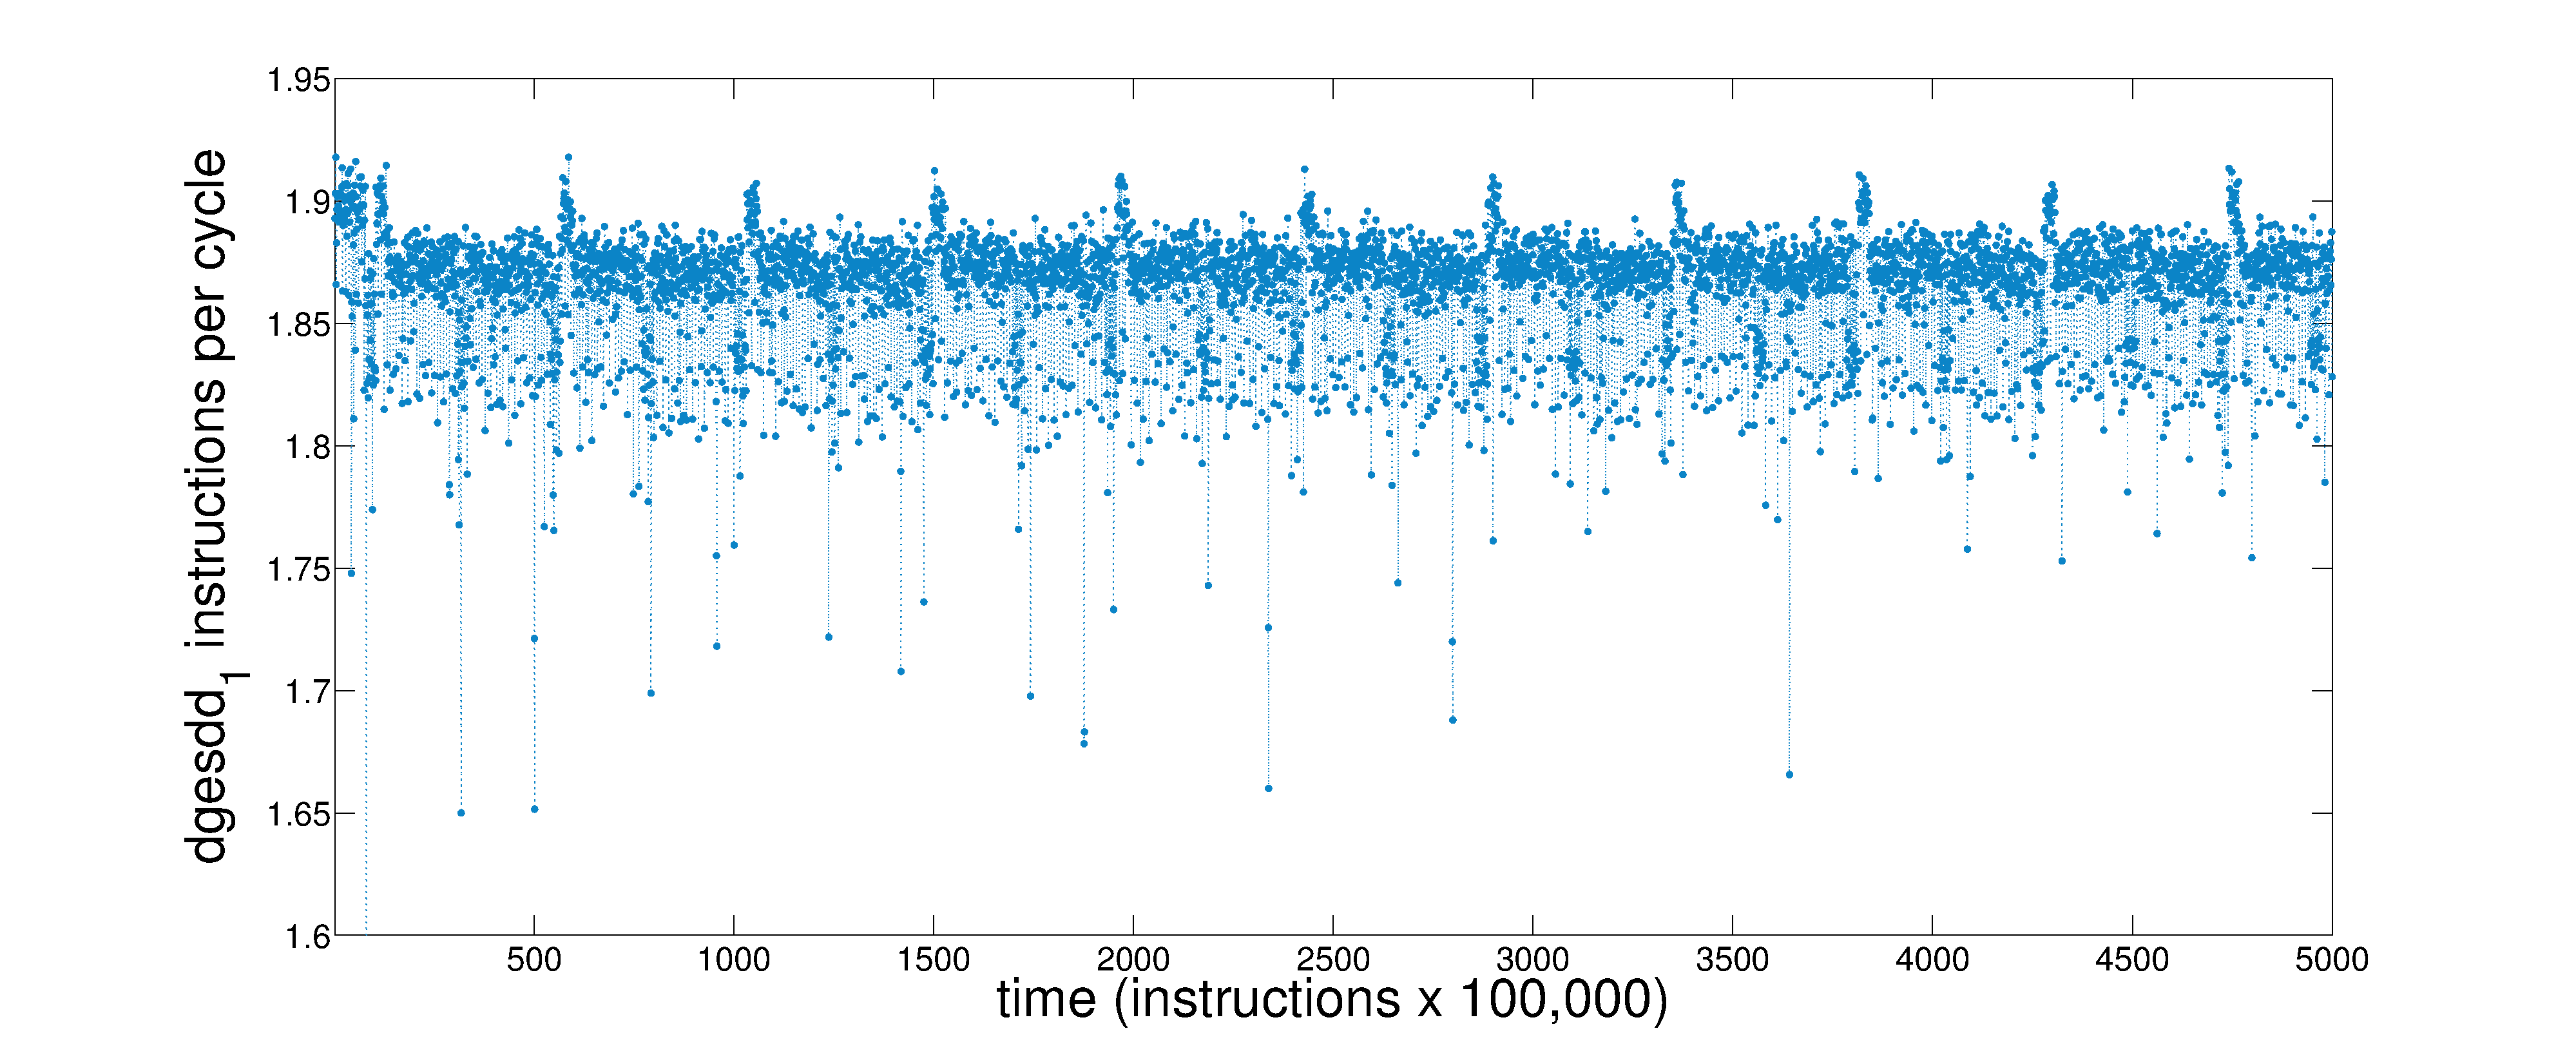
\includegraphics[width=\textwidth]{figs/svdonets2}
\caption{ For each of these, the word length used is $6$. The MASE values for LMA against ARIMA. The dashed line is the identity, delineating the traces for which either LMA or ARIMA performed better. All traces except those from \svd$_1$ lie above the line, indicating that LMA is better suited prediction method for the computer traces considered.}\label{fig:svdone-ts}  
\end{figure} 
As can be seen in Figure \ref{fig:svdone-ts}, \svdone has a highly unstructured small band on top, which is approximately 0.05 instructions per cycle wide. Approximately 80\% of the signal exists within this band of noise, this causes the WPE to be driven up as many words are being omitted by this band of the signal. The remaining 20\% of the signal are drops in instructions per cycle away from this band, ranging in size from 0.1 to 0.6 instructions per cycle\footnote{Some of the large drops are not shown for the sake of clarity of the smaller scale}. These drastic drops seem to happen every 5-7 points but the drop locations are inconsistent as well as the drops magnitude (ranging from 0.1-0.6 instructions per cycle). As discussed in Section \ref{sec:RWMethod} drops of this fashion are the bane of random walk forecasting. At every one of these drops a random walk predictor would produce two forecasts with an error 2-12 times the magnitude of the smaller band, i.e., about 40\% of the time the random walk forecast would predict with error 2-12 times the magnitude of the scale exhibited by $\approx$80\% of the signal. This inconsistency in random walk would cause cause random walk error to be high and as a result MASE scores to be artificially low. The combination of a band of noise with a high number of random drops is a weakness of this method which is present in \svdone and as a result makes this signal an outlier.


[[Joshua: I am not sure if this paragraph is strong enough or even worth having]]These results support that time series with low to moderate complexity ($0\le WPE \le 0.85$) can be predicted more efficiently than a na\"ive random walk \emph{and} that complexity can be qualitatively measured for a real-valued noisy time series using WPE. This will allow practitioners to stop spinning their wheels in the case of signals who are simply better predicted with a simple strategy like random walk. The analysis of these results illuminates an interesting point: The way structure, information and complexity are processed by a generating process plays a crucial role in the success of a given prediction scheme. 











%This portion should justify the following claim%%%%%%%%%%%%%%%%%%%%%%
%\item The way structure/information/complexity is processed internally by a given process plays a crucial role in predictability.
%%%%%%%%%%%%%%%%%%%%%%%%%






Comparing Figures~\ref{fig:lma_pred_vs_ent} and \ref{fig:arima_pred_vs_ent} also elucidates another key finding: usable and quantifiable predictive structure can be present in a time series without a prediction scheme being able to utilize it. In particular, information may be transferred from past to future through the present but because of the mechanism the underlying process uses to process that information  (e.g., linear or nonlinear) certain prediction strategies may be blind to or not be able to efficiently utilize this information. For example, consider \col, programs like this have been shown to exhibit deterministic chaos \cite{mytkowicz09}. If this were the case with \col, an out-of-the-box linear method like ARIMA would simply be ill-equipped to model and utilize the kind of structure present, as is evident in Figure \ref{fig:arima_pred_vs_ent}. In contrast, a nonlinear predictor like LMA which is built to handle deterministic chaos, can interpret and utilize this type of structure just fine. We believe that many of the shifts in forecast accuracy for low-to-moderate WPE programs between ARIMA and LMA is precisely happening for this reason: Just because there is forward information transfer, does not mean that an arbitrary predictor can interpret or utilize it, but luckily WPE can tell us when this structure is present as shown in Figure \ref{fig:lma_vs_arima}.

%In Figures~\ref{fig:lma_pred_vs_ent} and \ref{fig:arima_pred_vs_ent} we directly compare the performance of the LMA and ARIMA prediction methods (respectively) to the value of the weighted permutation entropy for all runs of each program under consideration. The LMA MASE values are largely similar to those of the best predictions, primarily because LMA often performed superior to ARIMA (and the na\"ive method). On the other hand, the ARIMA MASE values are largely uncorrelated with WPE values. As was hinted at while discussing the previous results, the fact that ARIMA is uncorrelated with WPE brings about an interesting perspective on information transfer and WPE. The WPE is sensitive to both linear and nonlinear structure. When you have a low WPE and a high ARIMA it could be that the structure WPE is picking up is simply nonlinear structure that LMA can handle but ARIMA cannot. So while ARIMA is consistently out performed by random walk,  there is plenty of structure present as suggested by WPE and taken advantage of by LMA but since it is nonlinear ARIMA can't take it into account and does bad.



%is in large part one of the major findings of this work. More specifically, say we tried to predict an arbitrary noisy real-valued time series with an ``out-of-the-box" prediction strategy like ARIMA as proposed in \cite{autoArima} and say we got inconsistent and bad forecasts, (i.e., perform worse than the na\"ive random walk strategy (MASE$>1$). How do we determine if the prediction strategy is not adequate for the prediction task, or if the signal is simply too complex to predict. If a signal is too complex and too little forward information transfer is present we may not be able to do better than the random walk, in which case we should not worry ourselves over finding a more complicated prediction strategy. However, if we measure the complexity to be low, $\textrm{WPE}<0.85$ (see Fig.~\ref{fig:pred_vs_wpe}) we can most likely do much better than the random walk and should search for more adequate prediction strategies. 




 


Other noteworthy features of the LMA and ARIMA results are the cluster locations
and distributions. The WPE values of each run of any particular program tend to
have little variance, leading to the clusters in
Figures~\ref{fig:arima_pred_vs_ent} and \ref{fig:lma_pred_vs_ent} to be fairly
constrained in the $y$ direction. For most traces, the LMA and ARIMA variance is
low as well, resulting is small, tight clusters. The ARIMA MASE values of the \col
traces, however, have a large variance resulting in the spread seen in
Figure~\ref{fig:arima_pred_vs_ent}. Not only are the MASE values of that cluster
bad, in that other predictors vastly outperform it, but they are inconsistent.
Furthermore, since LMA can predict nonlinear behavior while ARIMA cannot, we
see that the clusters in Figure ~\ref{fig:arima_pred_vs_ent} are mostly further to
the right than those in Figure~\ref{fig:lma_pred_vs_ent}.

